\section{Results}
\label{sec:results-hbn}

This section presents the results for our five proposed RQs. We highlight two P/R curves and focus our discussion on the AP results. However, all P/R curves and confidence interval graphs are currently available in our appendix alongside all experimental data~\citep{appendix}.

%------------------------------------------------

\subsection{RQ$_1$ Results: C{\footnotesize OMET} Stage 1 Performance}
\label{sub:results-rq1}

\begin{table}[h]
	\footnotesize
	\centering
	%	\small
	\caption{\footnotesize AP Results from Stages 1 \& 4 of \Comet. The given $p$ values from the Wilcoxon test measure the significance of performance variations between Stage 1, and Stage 4 of \Comets model compared to the median (Med.) baseline of IR/ML techniques. ``I=Net'' signifies the ``Industry-Net'' dataset.}
	
	\label{tab:stage1-4-results}
	
\begin{tabular}{@{}l|c|c|c|c|c|c|c@{}}
\toprule
\multicolumn{1}{c|}{\textbf{Dataset}} &
  \textbf{\begin{tabular}[c]{@{}c@{}}Best\\ Base.\end{tabular}} &
  \textbf{\begin{tabular}[c]{@{}c@{}}Med.\\ Base.\end{tabular}} &
  \textbf{std. Err} &
  \textbf{DL} &
  \textbf{St.1} &
  \textbf{std. Err} &
  \textbf{St.4} \\ \midrule
LibEst (Rq to Src)  & 0.69 & 0.55 & pm 0.008 & 0.28 & 0.63 & pm 0.006 & 0.64 \\
LibEst (Rq to Test) & 0.42 & 0.36 & pm 0.001 & 0.32 & 0.38 & pm 0.002 & 0.42 \\
eTour               & 0.40 & 0.30 & pm 0.011 & 0.05 & 0.05 & pm 0.002 & 0.36 \\
EBT                 & 0.17 & 0.14 & pm 0.005 & 0.07 & 0.07 & pm 0.001 & 0.17 \\
SMOS                & 0.29 & 0.25 & pm 0.003 & 0.16 & 0.16 & pm 0.001 & 0.27 \\
iTrust              & 0.17 & 0.13 & pm 0.006 & 0.01 & 0.01 & 0        & 0.17 \\ \bottomrule
\end{tabular}

\end{table}

The AP values for Stage 1 of \Comets HBN are provided in \tabref{tab:stage1-4-results} alongside the $p$ values for the Wilcoxon test between Comet and the median IR/ML baseline. The P/R curves for the iTrust dataset are illustrated in \figref{fig:pr1-results}. As \tabref{tab:stage1-4-results} indicates, Stage 1 of \Comet outperforms the median IR/ML baseline across all subjects, to a statistically significant degree according to the confidence intervals. In some cases, such as for iTrust, LibEST, and eTour, Stage 1 of \Comet \textit{significantly} outperforms the median IR/ML baseline, and approaches the performance of the \textit{best} IR/ML baseline. \figref{fig:pr1-results} illustrates the P/R curve for the iTrust project, with performance that outpaces the best IR/ML technique, particularly for lower recall values. \Comet also outperforms the state of the art DL approach across all subjects, likely because the DL approach had difficulty generalizing semantic relationships across datasets.

These results signal remarkably strong performance for \Comets Stage 1 model. Recall that, the Stage 1 model \textit{only} utilizes observations taken from the set of ten IR/ML techniques introduced in Sec. \ref{sub:study-rq1}, thus the fact that the Stage 1 model was able to consistently outperform the median IR/ML baselines and in some cases, nearly match the best IR/ML baseline. This indicates that \Comets HBN is capable of effectively combining the observations from the underlying IR/ML techniques for improved inference power. This is significant, as currently practitioners cannot know a-priori which IR/ML technique for traceability will perform best on a given project without pre-existing trace links. Thus, by combining the collective information of several IR techniques \Comets first stage HBN is able to perform \textit{\textbf{consistently well}}, achieving reasonably high performance \textit{\textbf{across projects}}, lending to the credibility of using Comet for projects that do not contain preexisting links. 

%------------------------------------------------

\subsection{RQ$_2$ Results: C{\footnotesize OMET} Stage 2 Performance}
\label{sub:results-rq2}

\begin{table}[h]
	\footnotesize
	\centering
	%	\small
	%\vspace{-0.0cm}
	\caption{\footnotesize AP Results from Stage 2 of \Comet with simulated expert feedback with error rates of 25\% and 50\%. The Baseline AP reported in this table is the median of the IR/ML techniques for the sampled links affected by feedback.}
	%\vspace{-1.0em}
	\label{tab:stage2-results}
	\setlength{\tabcolsep}{0.1em}
	
\begin{tabular}{@{}l|c|c|c|c|c|c@{}}
\toprule
\multicolumn{1}{c|}{\textbf{Dataset}} & \textbf{Baseline} & \textbf{St.1} & \textbf{St.2 (25\%E)} & \textbf{Baseline} & \textbf{St.1} & \textbf{St.2 (50\%E)} \\ \midrule
LibEst (Rq to Src)  & 0.52 & 0.65 & 0.96 & 0.52 & 0.65 & 0.64 \\
LibEst (Rq to Test) & 0.28 & 0.32 & 0.80 & 0.28 & 0.32 & 0.44 \\
eTour               & 0.48 & 0.60 & 0.66 & 0.48 & 0.60 & 0.39 \\
EBT                 & 0.20 & 0.22 & 0.38 & 0.20 & 0.22 & 0.24 \\
SMOS                & 0.18 & 0.17 & 0.39 & 0.18 & 0.17 & 0.17 \\
iTrust              & 0.12 & 0.15 & 0.25 & 0.12 & 0.15 & 0.10 \\ \bottomrule
\end{tabular}

%\vspace{0.35cm}
\end{table}
\begin{table}[h]
	\footnotesize
	\centering
	%	\small
	%\vspace{-0.7cm}
	\caption{\footnotesize AP Results from Stage 3 of \Comet for transitive links between requirements with $\tau$=0.55 and $\tau$=0.65. The baseline reported in this table is the median of the IR/ML techniques for links affected by transitive relationships.}
	%\vspace{-1.0em}
	\label{tab:stage3-results}
	\setlength{\tabcolsep}{0.1em}
	
\begin{tabular}{@{}l|c|c|c|c|c|c@{}}
\toprule
\multicolumn{1}{c|}{\textbf{Dataset}} & \textbf{Baseline} & \textbf{St.1} & \textbf{St.3 (tau=.55)} & \textbf{Baseline} & \textbf{St.1} & \textbf{St.2 (tau=.65)} \\ \midrule
LibEst (Rq to Src)  & 0.53 & 0.60 & 0.59 & 0.39 & 0.67 & 0.44 \\
LibEst (Rq to Test) & 0.38 & 0.40 & 0.38 & 0.18 & 0.19 & 0.22 \\
eTour               & 0.33 & 0.40 & 0.42 & 0.37 & 0.48 & 0.48 \\
EBT                 & 0.24 & 0.26 & 0.24 & 0.02 & 0.03 & 0.06 \\
SMOS                & 0.19 & 0.20 & 0.19 & 0.24 & 0.23 & 0.24 \\
iTrust              & 0.11 & 0.14 & 0.15 & -    & -    & -    \\ \bottomrule
\end{tabular}

\end{table}

The AP for for Stage 2 of \Comet across all subject programs for both 25\% and 50\% error rates is given in Table \ref{tab:stage2-results}. The results indicate that Stage 2 of \Comets HBN is able to effectively incorporate expert feedback to improve the accuracy of its trace link inferences, as the Stage 2 model dramatically outperforms the median (and best) IR/ML techniques as well as the first stage of the model, with a simulated error rate of 25\%.  Even for the larger error rate of 50\%, we see Stage 2 outperform Stage 1 for LibEST (Rq$\rightarrow$Src), LibEST (Rq$\rightarrow$Tests) and EBT, while it slightly underperforms the Stage 1 model for the other subjects. These results illustrate that Stage 2 of \Comets HBN is able to effectively utilize expert feedback to improve its inferences, even in the presence of significant noise.


\subsection{RQ$_3$ Results: C{\footnotesize OMET} Stage 3 Performance}
\label{sub:results-rq3}

\begin{figure}[h]
\centering

\begin{subfigure}{0.5\textwidth}
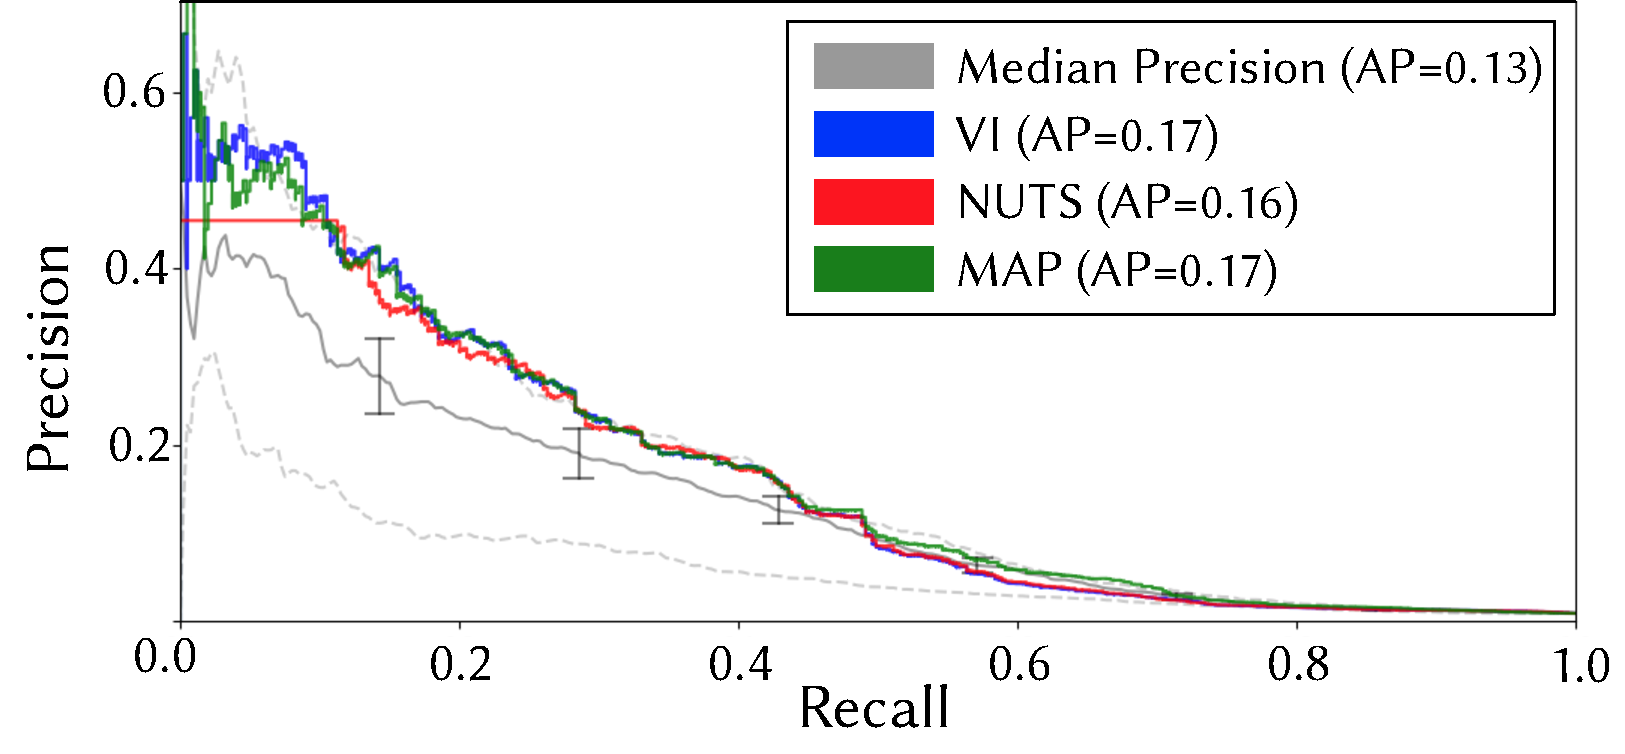
\includegraphics[clip,width=\textwidth]{graphics/chap_04-bayes/fig3_Stage1-single.pdf}
\caption{\footnotesize P/R Curve for iTrust for Stage 1.}
\label{fig:pr1-results}
\end{subfigure}

\begin{subfigure}{0.5\textwidth}
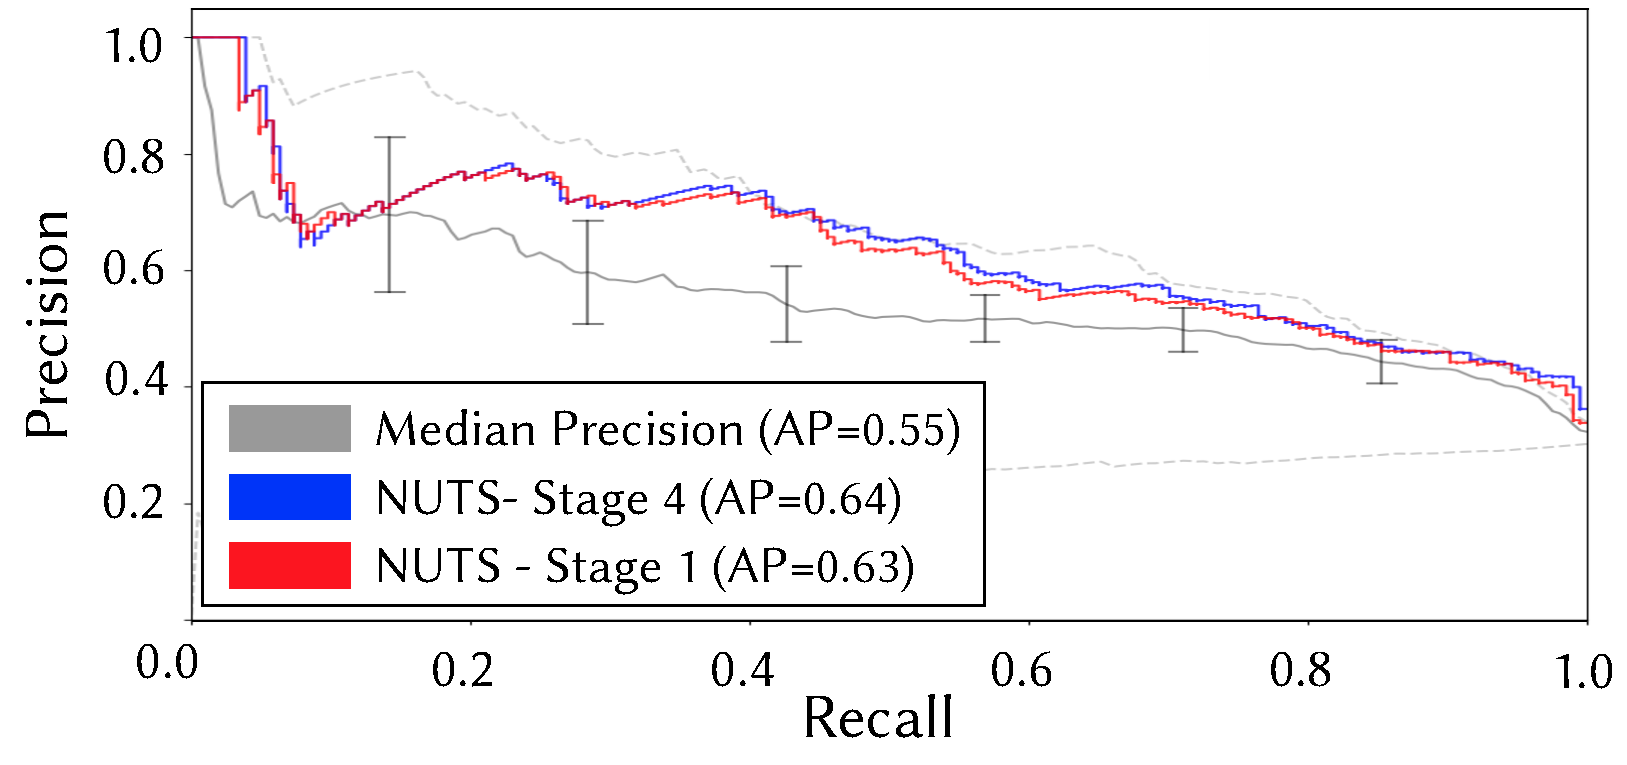
\includegraphics[clip,width=\textwidth]{graphics/chap_04-bayes/fig4_Stage4-single.pdf}
\caption{\footnotesize P/R Curve for I-Net (Req$\rightarrow$Src) for Stage 4.}
\label{fig:pr4-results}
\end{subfigure}

\caption{\footnotesize Selected P/R Curves for Stage 1 and Stage 4 of \Comet.  Solid grey line is median of the baseline IR/ML techniques, dotted grey lines are best and worst performing IR/ML techniques respectively.}

\end{figure}

The AP results for Stage 3 of \Comet, which incorporates transitive relationships between requirements, for both $\tau=0.55$ and $\tau=0.65$ are given in Table \ref{tab:stage3-results} (There were no transitive links in iTrust for $\tau=0.65$). This table also includes the median of the baseline IR/ML techniques, as well as the Comet Stage 1 model AP results, for the set of links affected by transitive relationships (hence the differing Stage 1 columns). The results show that, in general, for $\tau=0.65$ for \Comets Stage 3 model, the accuracy of \Comets inferred trace links improve, with four of the six datasets showing improvements. For $\tau=0.55$ the results generally exhibit similar or slightly worse performance compared to Stage 1.  The fact that the higher value of $\tau$ led to better performance improvements is not surprising, as this parameter essentially controls the \textit{degree of relatedness} required to consider transitive relationships. Thus, a higher value of $\tau$ means that only highly similar transitive requirement relationships are considered by \Comet's model. Using a lower value for this parameter might introduce noise by incorporating transitive relationships between artifacts that don't have as high a degree of similarity. 

The LibEST (Rq$\rightarrow$Src) dataset exhibited decreased performance for $\tau=0.65$, however this is likely because the requirements for this industrial dataset are based on formal format from the Internet Engineering Task Force (IETF). The somewhat repetitive nature of the language used in these requirements could lead to non-related requirements being transitively linked, leading to a decrease in performance. This suggests leveraging transitive relationships between requirements leads to larger performance gains for more unique language. Overall, our results indicate that \Comets Stage 3 model improves the accuracy of links for a majority of subjects.

%------------------------------------------------
\subsection{RQ$_4$ Results: C{\footnotesize OMET} Holistic Performance}
\label{sub:results-rq4}

The AP results for the the holistic \Comet (Stage 4) model are given in Table \ref{tab:stage1-4-results}. These results show that \Comets holistic model outperforms the baseline median IR/ML techniques, and Stage 1 for all subject programs. For three subjects (LibEST Req$\rightarrow$Src, EBT, and iTrust), Comet's holistic model matches or outperforms the best baseline IR/ML technique. \figref{fig:pr4-results} illustrates the P/R curve for the LibEST (Req$\rightarrow$Src) dataset, which shows that the performance gains in inference precision extend for a large range of recall values. The results of these experiments demonstrate that \Comets holistic model is able to effectively combine information from multiple sources to improve its trace link inference accuracy.


%------------------------------------------------
\subsection{RQ$_5$ Results: Industrial Case Study}
\label{sub:results-rq6}

\begin{figure}[h]
\centering
%\vspace{0.2cm}
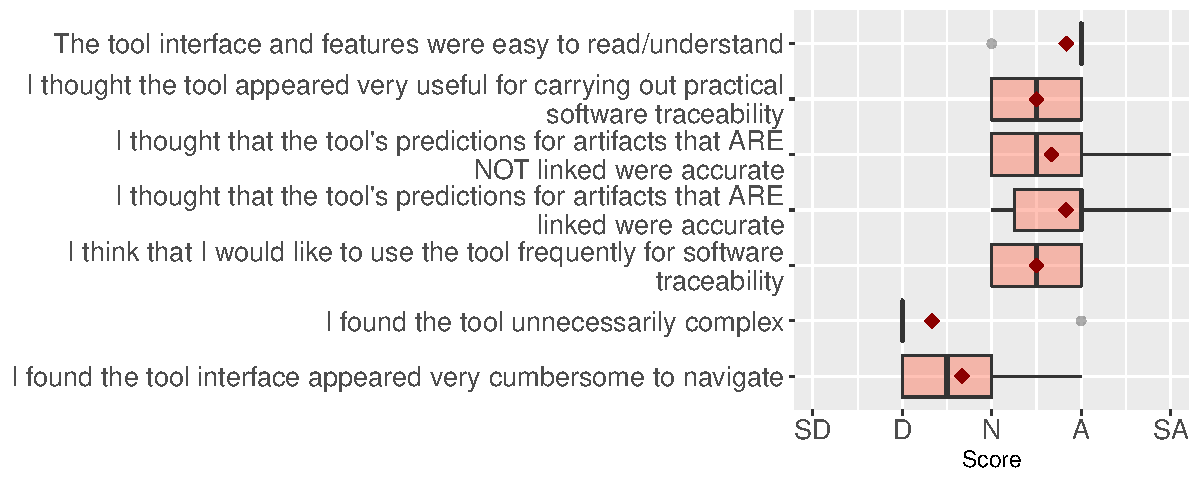
\includegraphics[width=\columnwidth]{graphics/chap_04-bayes/fig5_libest_boxplot.pdf}
%\vspace{-0.7cm}
\caption{Results for LibEST Case Study UX Questions}
%\vspace{-0.0cm}
\label{fig:LibEST-study}
%\vspace{-0.5cm}
\end{figure}

\figref{fig:LibEST-study} provides the responses to the likert-based UX questions from the six developers who work on the LibEST project after interacting with the \Comet plugin. Overall, the responses from these developers were quite positive. They generally agreed the \Comet plugin easy to use and understand, but more importantly, generally found the accuracy of the inferred links and non-links to be accurate. Additionally, we highlight representative responses to the user experience questions in this section, and provide the survey questions with response summaries in our online appendix~\citep{appendix}, in accordance with the NDA established with our industrial partner. Overall the developer responses were encouraging, indicating the practical need for approaches like \Comet. For instance, one developer stated their need for such a tool, \textit{``I really want a tool that could look at test cases and requirements and tell me the coverage. That way the team can know whether we are missing functionality or not.''} Another developer explained the need for a feature that incorporates developer feedback, stating the importance of the \textit{``ability to describe or explain how the code matches up with the code for future reference. Discussion/comments about such explanation as different developers might see links that others don't''}, whereas another developer stated, \textit{``Being able to provide feedback is useful and seeing it update the percentage immediately was nice.''}  This indicates that the support for developer feedback and responsiveness of the \Comet plugin inherently useful. Developers also found the traceability report to be useful, with most criticism suggesting practical UI improvements. For instance, developers appreciated \textit{``The fact that there were the three different options for viewing the traceability between different [artifacts]''}, and \textit{``The ability to bring up the specific requirement quickly in the same window.''}. These responses illustrate the utility that developers saw in the \Comet plugin. Given that these developers had little automated support for traceability tasks, they appreciated any automated assistance. 

We also collected feedback that validated the importance of the practical use cases that the \Comet plugin enabled. In these interviews, the teams generally stated that \Comet would be very useful for code auditing, as one manager stated that it would \textit{``allow compliance analysts to [inspect] links, look at the code and validate [the links]''}. Furthermore, a team responsible for security audits of systems found an interesting use case for \Comet that is often overlooked in traceability analysis. That is, they were interested in code and requirements that are \textit{not linked to any other artifact}, as such artifacts are likely to be suspicious and should be inspected further. In this case, \Comets inferences of non-links would be just as important as the inferences of links. Overall, the interviewed teams saw great promise in \Comet, and expressed interest in adoption.